% makeindex < aebpro_man.idx > aebpro_man.ind
\documentclass{article}
\usepackage[fleqn]{amsmath}
\usepackage[
    web={centertitlepage,designv,forcolorpaper,
         usesf,latextoc,pro}, %tight,
    eforms,aebxmp
]{aeb_pro}
\usepackage{graphicx,array}
\usepackage[dvipsone,!preview,!viewMagWin]{fitr}
\usepackage[js=restoreHookBlink,js=jmpHookBlink]{lmacs}

\usepackage[fortextbook,usecustomdesign,nomarginwrite]{eqexam}

%\usepackage{myriadpro}
\usepackage[altbullet]{lucidbry}

\renewcommand\allowFXDefault{false}


%\usepackage{makeidx}
%\makeindex
\usepackage{acroman}

\makeatletter
\def\eq@fititin#1{\noindent\unskip\nobreak\hfill\penalty50
    \hskip2em\hbox{}\nobreak\hfill#1}
\def\fitit{\eq@fititin{\exrtnlabelformat}}
\@mparswitchfalse\reversemarginpar
\def\meta#1{$\langle\textit{\texttt{#1}}\rangle$}

\makeatother
%\usepackage[active]{srcltx}

\urlstyle{rm}
\def\fitrpkg{\textsf{f{i}tr}}

\DeclareDocInfo
{
    university={\AcroTeX.Net},
    title={\texorpdfstring{The}{The manual for the} f{i}tr Package\texorpdfstring{\\
        Defining and Jumping to\\a Rectangular Destination}{}},
    author={D. P. Story},
    email={dpstory@acrotex.net},
    subject=Documentation for the fitr package,
    talksite={\url{www.acrotex.net}},
    version={1.0},
    Keywords={LaTeX,PDF,fitr,JavaScript,Adobe Acrobat},
    copyrightStatus=True,
    copyrightNotice={Copyright (C) \the\year, D. P. Story},
    copyrightInfoURL={http://www.acrotex.net}
}
\DeclareInitView{windowoptions={showtitle}}


\def\dps{$\hbox{$\mathfrak D$\kern-.3em\hbox{$\mathfrak P$}%
   \kern-.6em \hbox{$\mathcal S$}}$}

\universityLayout{fontsize=Large}
\titleLayout{fontsize=LARGE}
\authorLayout{fontsize=Large}
\tocLayout{fontsize=Large,color=aeb}
\sectionLayout{indent=-62.5pt,fontsize=large,color=aeb}
\subsectionLayout{indent=-31.25pt,color=aeb}
\subsubsectionLayout{indent=0pt,color=aeb}
\subsubDefaultDing{\texorpdfstring{$\bullet$}{\textrm\textbullet}}

%\pagestyle{empty}
\parindent0pt
\parskip\medskipamount


\definePath\bgPath{"C:/Users/Public/Documents/%
    ManualBGs/Manual_BG_Print_AeB.pdf"}
\begin{docassembly}
\addWatermarkFromFile({%
    bOnTop: false,
    cDIPath: \bgPath
})
\executeSave()
\end{docassembly}

\begin{document}

\maketitle

\selectColors{linkColor=black}
\tableofcontents
\selectColors{linkColor=webgreen}

\section{Introduction}

This package is an implementation of the \textbf{FitR} view-type
destination. The \textsl{PDF Reference} describes \textbf{FitR} as,
\begin{quote}
    Display the page designated by page, with its contents
    magnified just enough to fit the rectangle specified by the
    coordinates \textsl{left}, \textsl{bottom}, \textsl{right},
    and \textsl{top} entirely within the
    window both horizontally and vertically.
\end{quote}
The package supports the \textsf{dvips}, \textsf{dvipsone}, and
\textsf{pdftex}, \textsf{luatex}, \textsf{dvipdfm}, \textsf{dvipdfmx}, and
\textsf{xetex} applications, the first two assume that \textbf{Adobe
Distiller} is the PDF creator.

The only required packages are the \textsf{eforms} package (dated
2012/06/20 or later), which is part of the \textbf{AeB Bundle}, and
\textsf{collectbox} by Martin Scharrer, more on this package later, and
the ubiquitous \textsf{xcolor}.\footnote{The \textsf{eforms} package
itself brings in other packages, including \textsf{hyperref} and
\textsf{insdljs}.}

The package was developed in response to a user of the AeB Bundle who was
interested in developing documents for students with low vision; the idea
is to magnify regions of the document so the student can read more
comfortably. The demonstration files are \texttt{fitr\_demo.tex} which
illustrates the package and some special methods for people with low
vision, and \texttt{fitr\_minimal.tex}, which is the same demo file with
any and extra package stripped out.

\section{The Preamble and Package Options}

The minimal preamble for this package is
\begin{Verbatim}[xleftmargin=20pt,commandchars=!()]
\usepackage[!meta(driver),!meta(options)]{fitr}
\end{Verbatim}
The \textsf{hyperref} package is brought in through the \textsf{eforms} package.
Optionally, {\fitrpkg} can be used with other members of AeB (\textsf{web} and
\textsf{exerquiz}, for example).

Another package requirement is \textsf{collectbox} by Martin Scharrer;
quoting from the abstract of the documentation,
\begin{quote}
This package provides macros to collect and process an macro argument
(i.e. something which looks like a macro argument) as horizontal box
instead as a real macro argument. These ``arguments'' will be stored like
when using \cs{savebox}, \cs{sbox} or the \texttt{lrbox} environment and
allow verbatim or other special code. Instead of explicit braces also
implicit braces in the form of \cs{bgroup} and \cs{egroup} are supported.\dots
\end{quote}
The \cs{collectbox} command is used to collect the second argument of
\cs{jdRect}, see the discussion of \cs{jdRect} in Section~\ref*{jdRect}.
As a result, the second argument may contain verbatim text in it. Very cool.

The package has ten options: six driver options and four viewing
options.
\begin{itemize}
\item \textbf{Driver Options:} These are \texttt{dvips} (the default),
    \texttt{dvipsone}, and \texttt{pdftex} (which includes the use of
    lualatex), \texttt{dvipdfm}, \texttt{dvipdfmx}, and \texttt{xetex}. If you
    specify one of the first two, it is assumed that you are using
    \textbf{Adobe Distiller} as your PDF creator.

\item[] The \textsf{fitr} package checks whether the \textsf{web}
    package is loaded, if so, its uses the driver used by
    \textsf{web}; otherwise \textsf{fitr} auto-detects for
    \textsf{pdftex} and \textsf{xetex}. If no driver is passed, and
    neither \textsf{pdftex} nor \textsf{xetex} are detected, then
    \textsf{dvips} is the default driver.

\item \textbf{Viewing Options:} When you specify \texttt{preview}, the
bounding boxes of the buttons are shown in the dvi-previewer (or the PDF
document); you can turn off this preview by specifying \texttt{!preview}
(or removing \texttt{preview} entirely from the option list). The other
option type is \texttt{viewMagWin}, when this option the viewing window, a
rectangular region, becomes visible in the dvi-previewer (or in the PDF
document); specifying \texttt{!viewMagWin} turns off this type of preview.

\item[] The effects of the viewing options will be illustrated later in this
document, see \autoref{previewEx} on page~\pageref*{previewEx}.

\end{itemize}

\section{The one and only command}\label{jdRect}

The {\fitrpkg} has only one command, \cs{jdRect}, but there are two forms
of usage. \cs{jdRect} optionally creates a push button or link, and
optionally creates a viewing window. The term \emph{viewing window} refers
to a rectangular region that is created by the \textbf{FitR} destination
viewing specification, see \textbf{Table~8.2 Destination syntax} of the
\textsl{PDF Reference}, version 1.7. A \emph{named destination} is created
and is associated with the viewing window. When we jump to a viewing
window, this window is magnified to the largest extent possible. For
example, click on the either of the two displayed forms of the syntax for
\cs{jdRect}; after jumping to the viewing window, click on the same
display to return to the previous view.

%\previewtrue

There are two versions of \cs{jdRect}, the command itself, and a
\texttt{*} version, \cs{jdRect*}. The syntax follows, along with the
expected parameters.
\begin{quote}
    \jdRect*[adddestw=10bp,adddesth=10bp]{\cs{jdRect[\meta{key-values}]}}
\end{quote}
The above version is used to overlay a region with a button and view
window. No content is specified, but is defined by specifying the
\texttt{width} and \texttt{height}; it can be positioned using
\texttt{shift} and \texttt{lift}.

There is a \texttt{*}-version as well:
\begin{quote}
    \jdRect*[adddestw=10bp,adddesth=10bp]{\cs{jdRect*[\meta{key-values}]}\verb!{!\meta{content}\verb!}!}
\end{quote}
The second parameter \meta{content} is required when the \texttt{*} is
present. This version is meant to enclose \meta{content} within the button
and view window. The \texttt{width} and \texttt{height} keys are ignored,
but \texttt{shift} and \texttt{lift} are obeyed (though you may
\texttt{shift} or \texttt{lift} the button/view window away from the
content).

Before illustrating the \cs{jdRect} command, we first discuss its
key-value pairs.
\begin{itemize}
\item \texttt{lift=\meta{length}}: This key-value lifts (raises) the
    button/viewing window up (or down); for example,
    \texttt{lift=15pt} (or \texttt{lift=-15pt}). The default is a lift
    of \texttt{0pt}. See \autoref{displayEqEx} on page~\pageref*{displayEqEx}.

\item \texttt{shift=\meta{length}}: The amount of horizontal shift;
    positive to the right, negative to the left. For example,
    \texttt{shift=-1in} shifts the button/viewing window 1 inch to the
    left. The default is \texttt{0pt}. See
    \autoref{displayEqEx} on page~\pageref*{displayEqEx}.

\item \texttt{width=\meta{length}}: When using \cs{jdRect}---as
    opposed to \cs{jdRect*}---, the width of the button and viewing
    window is determined by the \texttt{width} key. For example
    \texttt{width=1in} creates a button/viewing window that is 1 inch
    wide. The value of this key is ignored when the \texttt{*} form of
    the \cs{jdRect} is used. The default value is \texttt{0pt}. This
    key is required when \texttt{*} is not present. See
    \autoref{displayEqEx} on page~\pageref*{displayEqEx}.

\item \texttt{height=\meta{length}}: Similar comments here as was made
    for the \texttt{width} key. This key is 0used to set the height of
    the button/viewing window. The default is 0pt. It is required when
    \texttt{*} is not present. See \autoref{displayEqEx} on
    page~\pageref*{displayEqEx}.

\item \texttt{ref=t|c|b}: The \texttt{ref} key-value pair determines
    the reference point of the button/viewing window. Permissible
    values are \texttt{t} top (the default), \texttt{c} center, and
    \texttt{b} bottom. This key is only obeyed with the \cs{jdRect*}
    form of the command; otherwise, a reference point of \texttt{b} is
    used.

\item \texttt{adddestw=\meta{length}}: The default is for the viewing window to have
the same dimensions as the underlying button. The \texttt{adddestw}
key-value pair is used to widen the viewing window; \texttt{adddestw=.2in}
widens the window by \texttt{.2in} on the left and \texttt{.2in} on the
right. See Figure~\ref*{bvw}, page~\pageref*{bvw}.

\item \texttt{adddesth=\meta{length}}: Similar to \texttt{adddestw} but for height.
The \texttt{adddesth}
key-value pair is used to increase the height the viewing window; \texttt{adddesth=.2in}
increases the height of the window by \texttt{.2in} on the top and \texttt{.2in} in the bottom.
See Figure~\ref*{bvw}, page~\pageref*{bvw}.
\begin{figure}[htb]
\begin{center}\setlength\fboxsep{0pt}
   \fbox{\parbox[c][.9in]{2.4in}
        {\vfill\hfil\fbox{\parbox[c][.5in]{2in}{\hfill\vfill}}\hfil\vfill}}\\[4pt]
        \caption{Button and Viewing Window}\label{bvw}
        {\small\texttt{width=2in,height=.5in,adddestw=.2in,adddesth=.2in}}
\end{center}
\end{figure}

\item \texttt{button=true|false}: \texttt{button} is a Boolean switch.
    If \texttt{true} (the default), \cs{jdRect} creates a push button.
    When the user pushes the button, the viewer zooms in to the view
    window. Clicking the same region again restores the previous view.

\item[] When \texttt{button} is \texttt{false}, the button is not created,
but the viewing window is still created. You can then jump to the viewing
window with a separate link or button. When \texttt{button=false}, use the
\texttt{dest} key to assigned a numbed destination to viewing window.
({\fitrpkg} automatically creates the definition names internally, they
are used by the buttons. If no button is created, name the destination so
your know its name and can reference it in link that jumps to that viewing
area.)


\item \texttt{link=jmp|restore} If \texttt{link} has a value, then
    {\fitrpkg} puts \texttt{button=false}. The \texttt{link} key is
    used to create jumps or restore actions to or from a viewing
    window. When \texttt{link=jmp} a jump action is created, the jump
    will be to the value of the \texttt{dest} key. If this is a pure
    link that jumps to another viewing window, then use the
    \texttt{nodest} key as well; no viewing window will be created
    around the link, as it is unlikely you'll want to jump to a link.

\def\RungePic{\kern0pt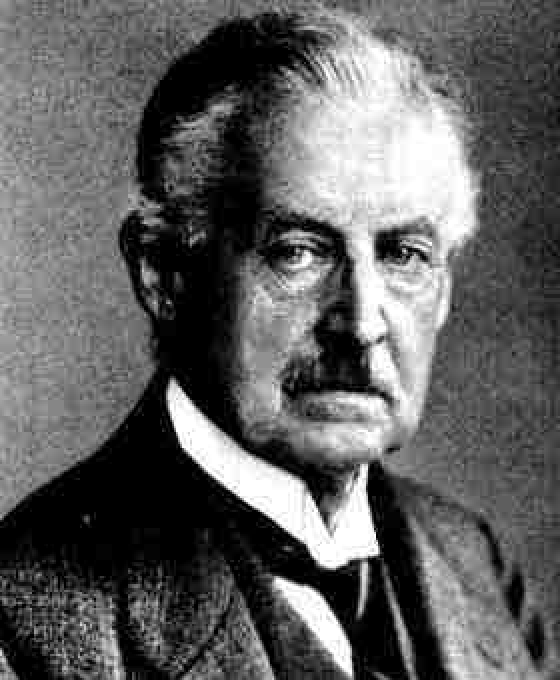
\includegraphics[width=\marginparwidth]{runge}}
\def\jrOpts#1#2{link=#1,dest=#2}

\item[] For example click on the link
\textbf{\jdRect*[nodest,\jrOpts{jmp}{rungePic},adddestw=10,adddesth=10]{Carl Runge}}%
\marginpar{\jdRect*[\jrOpts{restore}{rungePic},adddestw=\marginparsep,
adddesth=\marginparpush]{\parbox[t]{\marginparwidth}{\RungePic\\
\normalcolor\centering\footnotesize\textsf{Carl Runge}}}} and jump to
the picture of Runge in the margin. Click on the picture of Runge and
return to the previous view.

The jump to the picture from the text ``Carl Runge'' is as follows:
\begin{Verbatim}[xleftmargin=20pt]
\jdRect*[nodest,link=jmp,dest=rungePic,
adddestw=10bp,adddesth=10bp]{Carl Runge}
\end{Verbatim}
The important options are \texttt{nodest,link=jmp,dest=rungePic};
no (named) viewing window is created, we want to create a jump link here,
the destination of the jump link is the destination \texttt{rungePic}.

\item[] The color of the link is determined by \cs{@linkcolor}, a \textsf{hyperref}
command that holds a named color. This can be redefined at anytime,
directly using
\begin{Verbatim}[xleftmargin=20pt]
\makeatletter
\def\@linkcolor{blue}
\makeatother
\end{Verbatim}
or, if you are using the \texttt{pro} option with the \textsf{web}
package, you can say,
\begin{Verbatim}[xleftmargin=20pt]
\selectColors{linkColor=red}
\end{Verbatim}
When using the \textsf{web} package, the default is \texttt{webgreen}.

\item[] The action to restore the previous view is as follows:
\begin{Verbatim}[xleftmargin=20pt]
\marginpar{\jdRect*[link=restore,dest=rungePic,
    adddestw=\marginparsep,adddesth=\marginparpush
    ]{\parbox[t]{\marginparwidth}{\RungePic\\
    \normalcolor\centering\footnotesize\textsf{Carl Runge}}}}
\end{Verbatim}
The picture is placed in the margin using \cs{marginpar}; the command
\cs{RungePic} is a convenience macro that uses \cs{includegraphics} in
import the picture. The important options are
\texttt{link=restore,dest=rungePic}, this first key-value pair causes
\cs{jdRect} to create a restore link, the second one says to create a
viewing window with a name of \texttt{rungePic}, this is the
destination the Carl Runge link jumps to.


\item \texttt{nodest}: A Boolean switch whose default value is
    \texttt{false}. When \texttt{nodest} is used (making the switch a
    value of \texttt{true}), no viewing window is created.

\item \texttt{dest=\meta{name}}: This key is a way of explicitly naming the
    viewing window (the destination). The destination is normally
    automatically generated when \texttt{button=true}, this key is
    used with the \texttt{link} key, as illustrated above.
\item \texttt{allowFX}: A Boolean switch (of sorts). The \texttt{fitr}
    allows for special effects (FX) when a viewing window is jumped to
    and when the view is restored. The default value of
    \texttt{allowFX} is \texttt{true} allow special effects if there
    is any defined. By saying \texttt{allowFX=false}, no special
    effects are used, even if some are defined.

\item[] An example of special effects you say? Try clicking on the
    Pythagorean Theorem
    \jdRect*[allowFX,adddestw=10bp,adddesth=10bp]{$ a^2 + b^2 = c^2 $}
\end{itemize}

\section{Some Examples}

\everymath{\displaystyle}

In this section, several examples are presented that illustrate the
options of \cs{jdRect}.

\begin{example}\label{previewEx}\previewtrue\viewMagWintrue
\textbf{Illustrate Preview Rectangles.} The \texttt{preview} and
\texttt{viewMagWin} options just set Boolean switches. In this example, we
manually gives these switches a value of \texttt{true}
(\cs{previewtrue}\cs{viewMagWintrue}). Take a close look at the following
function
\jdRect*{$ f(x) = \frac{1}{\sqrt{2\pi}}\int_{-\infty}^x e^{-t^2/2}\,\text{d}t$},
or the more general form
\jdRect*[adddestw=20bp,adddesth=10bp]{$ f(x;\mu;\sigma) = \frac{1}{\sigma\sqrt{2\pi}}\int_{-\infty}^x e^{-\frac{(t-\mu)^2}{2\sigma^2}}\,\text{d}t$}
The preview rectangles are shown: For the one on the left, the dimensions
of the push button and the viewing rectangle are the same; for one on the
right, the dimensions of the viewing window have been increased by
using \texttt{adddestw=20bp,adddesth=10bp}. When you jump to each of these
viewing windows, you the one on the left is magnified much more than the
one on the right; the larger viewing window allows the user to see some of
the surrounding text.\fitit
\end{example}

\begin{example}\label{displayEqEx}
\textbf{Display Math.} Displayed math presents a problem. We take the
following set of equations to illustrate.

Suppose we want to classify third order \textsf{Runge-Kutta} type methods.
Start with
\begin{align*}
\jdRect[height=1.3in,width=2.6in,lift=16pt,shift=-15pt,
    adddestw=10bp,adddesth=10bp]
K_1 &= hf(t_n, y_n)\\
K_2 &= hf(t_n +r h, y_n+aK_1)\\
K_3 &= hf(t_n +s h, y_n+bK_1+cK_2)\\
K &= w_1 K_1+ w_2 K_2+ w_3 K_3\\
y_{n+1} &= y_n+K
\end{align*}
Find the system of equations satisfied by
\jdRect*[adddestw=10,adddesth=10]{$r,s, a, b, c, w_1, w_2, w_3$}
that will make the above algorithm a third order method.

The verbatim listing of this set of aligned equations is
\begin{Verbatim}[xleftmargin=20pt,numbers=left]
\begin{align*}
\jdRect[height=1.3in,width=2.6in,lift=16pt,shift=-15pt,
    adddestw=10bp,adddesth=10bp]
K_1 &= hf(t_n, y_n)\\
K_2 &= hf(t_n +r h, y_n+aK_1)\\
K_3 &= hf(t_n +s h, y_n+bK_1+cK_2)\\
K &= w_1 K_1+ w_2 K_2+ w_3 K_3\\
y_{n+1} &= y_n+K
\end{align*}
\end{Verbatim}
This is an example of \cs{jdRect} (the non-\texttt{*} version), so there
is no second argument.  In this case, we create our button dimensions
using \texttt{height=1.3in,width=2.6in}, line~(2). Note the positioning
of the \cs{jdRect} command, the upper-left point of the display. We then
use \texttt{lift=16pt,shift=-15pt} to move the button around to cover the
equations, line~(2); finally, we increase the dimensions of the viewing
window in line~(3) with \texttt{adddestw=10bp,adddesth=10bp}. Now, how
were the values of these keys determined? By trial and error, while the
\texttt{preview} and \texttt{viewMagWin} options were in effect. Below are
the same equations with \cs{previewtrue} and \cs{viewMagWintrue}, locally
invoked:\previewtrue\viewMagWintrue
\begin{align*}
\jdRect[height=1.3in,width=2.6in,lift=16pt,shift=-15pt,
    adddestw=10bp,adddesth=10bp]
K_1 &= hf(t_n, y_n)\\
K_2 &= hf(t_n +r h, y_n+aK_1)\\
K_3 &= hf(t_n +s h, y_n+bK_1+cK_2)\\
K &= w_1 K_1+ w_2 K_2+ w_3 K_3\\
y_{n+1} &= y_n+K
\end{align*}
The preview rectangles do not take up any {\TeX} space, so they overlap
parts of the paragraph content. When you zoom in, you'll see part of the
part of the word ``invoked:'', as seen in the upper-left corner, at least
according to the viewing window preview. Is it so?

After you've set the position of the rectangles, and after all changes
have been made to the underlying content, you don't need the preview
modes.\fitit
\end{example}

\begin{example}\label{CustomAppr}
\textbf{Customizing the appearance.} The properties of the underlying push button
is to be visible, but does not print. The background and the border are
transparent.  The default properties are passed to the push button using a
presets command:
\begin{Verbatim}[xleftmargin=20pt]
\newcommand{\overlayPresets}{\H{I}\BG{}\BC{}\S{S}}
\end{Verbatim}
See the \textsf{eforms} manual for the meaning of these cryptic symbols.
You can modify these settings locally, within a group, or globally. In
this example, we change the border to red dashed line. We redefine
\cs{overlayPresets} as follows:
\begin{Verbatim}[numbers=left,xleftmargin=20pt]
\renewcommand{\overlayPresets}{\H{I}\BG{}\BC{red}\S{D}}
\end{Verbatim}
\renewcommand{\overlayPresets}{\H{I}\BG{}\BC{red}\S{D}}%
The changes are in line~(2), we say \verb!\BC{red}! (the \textsf{xcolor} package is
required here for named colors; otherwise, we would say \verb~\BC{1 0 0}~),
and we've change \verb!\S{S}! to \verb~\S{D}~, which gives a dashed
(\texttt{D}) border as opposed to a solid (\texttt{S}) border. Now to
illustrate this. My name is \jdRect*{D. P. Story!}; lets increase the
viewing window, shall we? My name is \jdRect*[adddestw=10bp,adddesth=10bp]{D. P.
Story!}. Keep in mind that we are overlaying a push button; if you want
the underlying text to have a color, you need to color it yourself:
\jdRect*[adddestw=10bp,adddesth=10bp]{\textcolor{blue}{D. P. Story}!}
This last button has code,
\begin{Verbatim}[xleftmargin=20pt]
\jdRect*[adddestw=10bp,adddesth=10bp]%
    {\textcolor{blue}{D. P. Story}!}
\end{Verbatim}
As the changes to the preset appearance are inside a group, after this
example (environment)) \cs{overlayPresets} will revert to its definition
that was in effect outside the example.\fitit
\end{example}

\section{Special Effects}

For the standard set up, where there is a push button that overlays the
content along with the viewing window is jumps to, there are two
JavaScript ``hooks'' that can be exploited
\begin{itemize}
    \item \texttt{overlayJmpHook()} is an undefined JavaScript
        function that is executed after the jump to the viewing
        window. (It is enclosed in a \texttt{try/catch} construct that
        catches the error thrown.) The document author can define
        \texttt{overlayJmpHook()} to perform some action following the
        jump. The distribution of {\fitrpkg} comes with one
        definition, \texttt{jmpHookBlink.js}, which blinks the border
        following the jump.
    \item \texttt{overlayRestoreHook()} is an undefined JavaScript
        function that is executed following the restored view action.
        The document author needs to make a custom definition if
        special effects are desired. The distribution of {\fitrpkg}
        comes with one definition, \texttt{restoreHookBlink.js},
        which blinks the border following the restore action.
\end{itemize}
The preamble of this document says,
\begin{Verbatim}[xleftmargin=20pt]
\usepackage[js=restoreHookBlink,js=jmpHookBlink]{lmacs}
\end{Verbatim}
The \textsf{lmacs} package is a new package I made available to CTAN, its
a simple package that imports files with extensions of \texttt{.def}, \texttt{.cfg}, and
\texttt{.js}. We import \texttt{restoreHookBlink.js} and
\texttt{jmpHookBlink.js} using a key-value method, where the key is one of
the supported extensions; thus \texttt{js=restoreHookBlink} will import
the file texttt{restoreHookBlink.js} if it exists. By the way, another
nice feature of \textsf{lmacs} is that you can prefix an exclamation point
(!) to cancel out that import, for example, if we wanted to use \texttt{jmpHookBlink}
but not \texttt{restoreHookBlink} we say
\begin{Verbatim}[xleftmargin=20pt]
\usepackage[!js=restoreHookBlink,js=jmpHookBlink]{lmacs}
\end{Verbatim}

\begin{example}\label{fx}\renewcommand{\overlayPresets}{\H{I}\BG{}\BC{blue}\S{D}}%
\textbf{Special Effects.} Jump to the
\jdRect*[allowFX,adddestw=10bp,adddesth=10bp]{{\fitrpkg} Package!}

The verbatim listing is
\begin{Verbatim}[xleftmargin=20pt,numbers=left]
\renewcommand{\overlayPresets}{\H{I}\BG{}\BC{blue}\S{D}}%
...
Jump to the \jdRect*[allowFX,adddestw=10bp,adddesth=10bp]%
    {{\fitrpkg} Package!}
\end{Verbatim}
We redefined the \cs{overlayPresets} command, choosing an initial border
of blue. In line~(4), I've used \texttt{allowFX}, this key does not
normally to appear in the option list, its default value is normally
\texttt{true};  however, for this document, the following definition was
made in the preamble
\begin{Verbatim}[xleftmargin=20pt]
\renewcommand\allowFXDefault{false}
\end{Verbatim}
This (re)definition of \cs{allowFXDefault} sets the default value of
\texttt{allowFX} to \texttt{false}. This was done so the special effects
JavaScript functions could be imported (using \texttt{lmacs}) but their
effects would not be seen, by default. To see their effect, we have to
explicitly put \texttt{allowFX} to \texttt{true}, which is what the single
key does. (Or, you can say \texttt{allowFX=true}, but that is five more key
presses.)\fitit
\end{example}

Now, I simply must get back to my retirement. \dps

\end{document}
